\documentclass[tikz,border=10pt]{standalone}
\usetikzlibrary{shapes.geometric, arrows.meta}

\tikzset{
    block/.style={rectangle, draw, text width=5em, text centered, minimum height=4ex},
    line/.style={draw, thick, -Stealth, shorten >=2pt},
    decision/.style={diamond, draw, text width=5em, text badly centered, node distance=3cm, inner sep=0pt}
}

\begin{document}
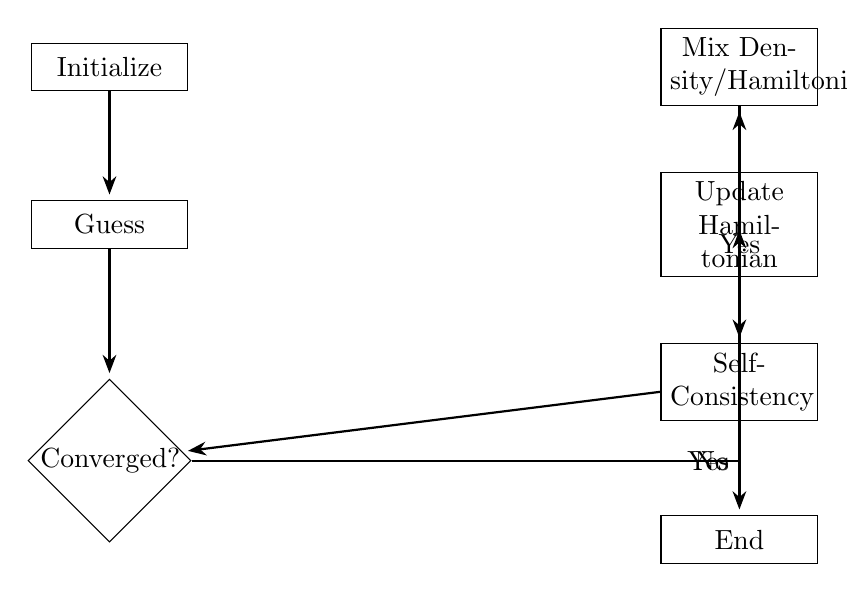
\begin{tikzpicture}[node distance = 2cm]

    % Nodes
    \node [block] (Initialize) {Initialize};
    \node [block, below of=Initialize] (Guess) {Guess};
    \node [decision, below of=Guess] (ConvergenceCheck) {Converged?};
    \node [block, right of=Initialize, xshift=6cm] (MixingStep) {Mix Density/Hamiltonian};
    \node [block, below of=MixingStep] (UpdateHamiltonian) {Update Hamiltonian};
    \node [block, below of=UpdateHamiltonian] (SelfConsistency) {Self-Consistency};
    \node [block, below of=SelfConsistency] (End) {End};

    % Edges
    \path [line] (Initialize) -- (Guess);
    \path [line] (Guess) -- (ConvergenceCheck);
    \path [line] (ConvergenceCheck) -| node[anchor=east] {No} (MixingStep);
    \path [line] (MixingStep) |- node[anchor=north] {Yes} (UpdateHamiltonian);
    \path [line] (UpdateHamiltonian) -- (SelfConsistency);
    \path [line] (SelfConsistency) -- (ConvergenceCheck);
    \path [line] (ConvergenceCheck) -| node[anchor=east] {Yes} (End);

\end{tikzpicture}
\end{document}